\documentclass[12pt]{article}
\usepackage{fullpage}
\usepackage{lastpage}
\usepackage{fancyhdr}
\pagestyle{fancy}

\addtolength{\topmargin}{-0.25in}
\usepackage{graphicx,tikz}	
\usepackage{tkz-euclide}
\usetkzobj{all}
\usetikzlibrary{calc}
\usepackage{array, multicol}
\usepackage{amsmath}

\everymath{\displaystyle}

\fancypagestyle{plain}{
	\fancyhf{}
	\addtolength{\headheight}{2.92\baselineskip}
	\lhead{\bf Quiz 6: Inverses and Related Rates \\
		\S 3.10-3.11 
		}
	\rhead{\bf MATH 2554 (Calculus I) \\
		%\vspace{0.5pc}
		due Tues 15 Mar 2016}
	\rfoot{Quiz 6 p.\thepage\ (of \pageref{LastPage})}
	}
\fancyhf{}
\renewcommand{\headrulewidth}{0pt}

\title{%\flushleft\vspace{-1.5pc}\Large
	%\bf Quiz 1: The Idea of Limits ($\textstyle\oint$2.1-2.2)
	}
\author{}
\date{}

\rfoot{Quiz 6 p.\thepage\ (of \pageref{LastPage})}

% % % % %
\begin{document}
\maketitle

\vspace{-7pc}
\noindent{\bf Directions:} This quiz is due on Tuesday, 15 March, 2016 at the beginning of your drill.  You may use your brain, notes, book, or other humans to complete your work.  \textbf{Your solutions must be on a separate sheet of paper, in order, stapled, de-fringed, and legible with your name on the top right corner of the first page.}  If you fail to meet any of these requirements, you will receive a zero.  Each question is worth one point, and will be graded as correct or not correct (all or nothing).

\noindent\hrulefill

\begin{enumerate}
% % %
\item {\bf (1 pt)} Find $f'(x)$, given $f(x)=\frac{\sec x\sin^2{(\tan^{-1}{(\ln x)})}}{\log_{6}{(e^{x^2\csc^{-1}{(\pi x)}})}}$.  You don't have to simplify.

% % %
\item Let $g(x)=\frac{x}{x+5}$.
	\begin{enumerate}
	\item {\bf (1 pt)} Find $g^{-1}(x)$.
	\item {\bf (1 pt)} Find $(g^{-1})'(x)$ and check that it is equal to $\frac{1}{g'(u)}$, where, after taking the derivative substitute $g^{-1}(x)$ for $u$.
	\end{enumerate}

% % %
\item \emph{(\S 3.10 \#68)} A biologist standing at the bottom of an 80-foot vertical cliff watches a peregrine falcon dive from the top of the cliff at a 45$^{\circ}$ angle from the horizontal.
\begin{center}
\includegraphics[scale=0.625]{Q6pic1}
\end{center}
\begin{enumerate}
	\item {\bf (1 pt)} Use the picture to write an expression for $\theta$ as a function of $h$.
	\item {\bf (1 pt)} What is the rate of change of $\theta$ with respect to the bird's height when it is 60 feet above ground?
\end{enumerate}

\newpage
% % %
\item %\emph{(Stewart\footnote{
%Stewart, J., \emph{Calculus: Single Variable Calculus}, 8th Edition.
%}
 %\S 2.8 \#21)} 
 The altitude (height) of a triangle is increasing at a rate of 1 cm/min while the area of the triangle is increasing at a rate of 2 cm$^{\text{2}}$/min.  Go through the following steps to answer:
\vspace{-0.5pc}
\begin{center}
\textbf{
What is the rate at which the base of the triangle is changing, when the altitude is 10 cm and the area is 100 cm$^{\text{2}}$?
}
\end{center}
Let $t$ denote time (min) and let $A$ denote the area of the triangle (cm$^{\text{2}}$/min).  Below is the triangle with the altitude and base named:
\vspace{-1pc}
\begin{center}
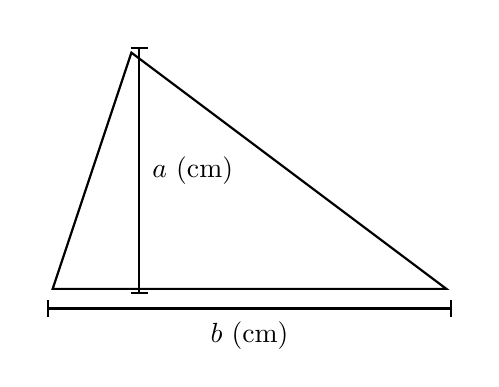
\begin{tikzpicture}[thick]
% draw the triangle:
	\coordinate (O) at (0,0);
	\coordinate (A) at (5,0);
	\coordinate (B) at (1,3);
	\draw (O)--(A)--(B)--cycle;
% identify some points of interest:
	\node (O') at ($(O)-(0.2,0.25)$){};
	\node (A') at ($(A)-(-0.2,0.25)$){};
	\node (B') at ($(B)+(0.1,0.2)$){};
	\node (bisect) at ($(O)!(B)!(A)$){};
	\node (bisect') at ($(bisect)+(0.1,-0.2)$){};
% draw lines and labels	
	\draw[|-|] (O') -- (A');
	%\draw[|-|] (O) -- (A);
	\tkzLabelSegment[below=1pt](O',A'){$b$ (cm)};
	\draw[|-|] (B') -- (bisect');
	%\draw[|-|] (B) -- (bisect);
	\tkzLabelSegment[right=1pt](B',bisect'){$a$ (cm)}
\end{tikzpicture}
\end{center}
\vspace{-1.5pc}
\begin{enumerate}
	\item {\bf (1 pt)} Translate the following information into mathematical expressions using the variables $b,a,t,A$.
		\begin{itemize}
		\item ``The altitude (height) of a triangle is increasing at a rate of 1 cm/min"
		\item ``the area of the triangle is increasing at a rate of 2 cm$^{\text{2}}$/min"
		\item ``rate at which the base of the triangle is changing"
		\item ``altitude is 10 cm"
		\item ``area is 100 cm$^{\text{2}}$"
		\end{itemize}
	\item {\bf (1 pt)} Use the picture to write an equation that includes the variables $a,b,A$.  Solve for $b$.  Then use implicit differentiation to solve for $\frac{db}{dt}$.
	\item {\bf (1 pt)} What is $\left.\frac{db}{dt}\right|_{\substack{h\,=10\text{ cm}\hfill \\ A=100\text{ cm}^2}\hfill}$?
\end{enumerate}

\vspace{1pc}
% % %
\item[] \hspace{-16pt}Use related rates, as above, to solve the following problems:
%\begin{enumerate}
\item {\bf (1 pt)} %\emph{(Stewart \S 6.6 \#49)} 
A ladder 10 ft long leans against a vertical wall.  If the bottom of the ladder slides away from the base of the wall at a speed of 2 ft/sec, how fast is the angle between the ladder and the wall changing when the bottom of the ladder is 6 ft from the base of the wall?
	
% % % 
\item {\bf (1 pt)} %\emph{(Stewart \S 2.8 \#50)}
 The minute hand on a clock is 8 in long and the hour hand is 4 in long.  How fast is the distance between the tips of the hands changing at 1 o'clock?  \textit{Hint: Use the Law of Cosines.}
%\end{enumerate}	

% % % % %
\end{enumerate}
\end{document}